
\documentclass[tikz]{standalone}
\usepackage{graphicx}
\usepackage{lmodern}
\usepackage{amsmath, amssymb, amsfonts}
\usetikzlibrary{calc}
\newcommand{\R}{\mathcal{R}}

\begin{document}
	
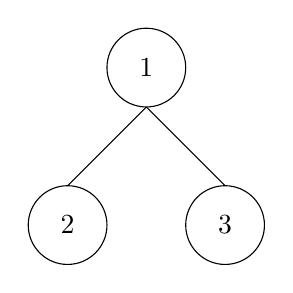
\begin{tikzpicture}
\draw (0, 4) circle (0.5);
\node at (0, 4) {$1$};

\draw (-1, 2) circle (0.5);
\node at (-1, 2) {$2$};

\draw (1, 2) circle (0.5);
\node at (1,2) {$3$};

\draw (0,3.5) -- (-1, 2.5);
\draw (0,3.5) -- (1, 2.5);

\end{tikzpicture}

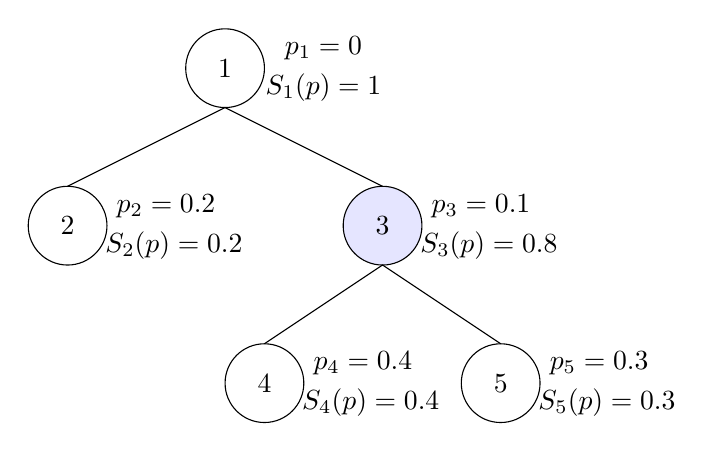
\begin{tikzpicture}
%node 1
\draw (0, 4) circle (0.5);
\node at (0, 4) {$1$};
\node at (1.25, 4.25) {$p_1 = 0$};
\node at (1.25, 3.75) {$S_1(p) = 1$};

\draw (-2, 2) circle (0.5);
\node at (-2, 2) {$2$};
\node at (-0.75, 2.25) {$p_2 = 0.2$};
\node at (-0.65, 1.75) {$S_2(p) = 0.2$};

\draw [fill=blue, fill opacity = 0.1] (2, 2) circle (0.5);
\node at (2,2) {$3$};
\node at (3.25, 2.25) {$p_3 = 0.1$};
\node at (3.35, 1.75) {$S_3(p) = 0.8$};

\draw (.5,0) circle (0.5);
\node at (.5,0) {$4$};
\node at (1.75, .25) {$p_4 = 0.4$};
\node at (1.85, -.25) {$S_4(p) = 0.4$};

\draw (3.5,0) circle (0.5);
\node at (3.5,0) {$5$};
\node at (4.75, .25) {$p_5 = 0.3$};
\node at (4.85, -.25) {$S_5(p) = 0.3$};

\draw (2, 2.5) -- (0,3.5) -- (-2, 2.5);
\draw (0.5, 0.5) -- (2,1.5) -- (3.5, .5);

\end{tikzpicture}

%geometrically calc original top k
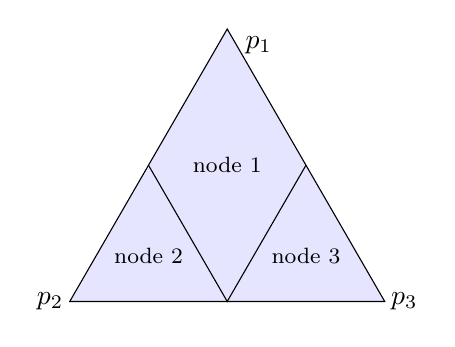
\begin{tikzpicture}
\path[fill=blue, opacity = 0.1] (2,0) -- (-2,0) -- (0,3.46) -- cycle;
%label outcomes
\node at (-9/4, 0) {$p_2$};
\node at (2/5, 3.25) {$p_1$};
\node at (9/4, 0) {$p_3$};
%level sets
\draw (-1, 1.73) -- (0,0) -- (1, 1.73) ; 
\node at (0, 1.73) {\footnotesize node $1$};

\node at (-1, 1.73 / 3) {\footnotesize node $2$};
\node at (1, 1.73 / 3) {\footnotesize node $3$};

\draw (2,0) -- (-2,0) -- (0,3.46) -- cycle;

\end{tikzpicture}




\end{document}
%%% Local Variables:
%%% mode: latex
%%% TeX-master: t
%%% End:
